\chapter{微分与扰动分析}
\label{chap:differential-perturbation-analysis}

测量误差、舍入误差或数据的轻微变化，都会让输入偏离理想值。第~\ref{chap:condition-and-spectral-perturbation}章已经不借助微分，直接比较精确变化$F(\bm x+\bm h)-F(\bm x)$，得到线性作用的条件数和谱的有限扰动界；这些界对一切方向取最坏情形。前三章则给出了另一种工具：微分把变化分成对$\bm h$线性的一阶响应和余项。本章把两者结合起来，回答三个问题：沿指定方向改变输入时，输出的一阶响应是什么；在所有允许方向中，误差最多被放大多少倍；对给定的有限步长，线性预测还差多少。

第一节对一般可微映射回答后两个问题。局部条件数用有限变化定义，可微时等于微分在允许方向子空间上的算子范数；余项界则需要导数沿整条扰动线段的变化，得到带明确常数的二次估计。这一节建立的是分析方法，不依赖具体运算。

后两节把这套方法用于矩阵。第二节调用第~\ref{chap:matrix-differentiation}章的微分公式与精确增量，逐个估计基本运算、求逆、行列式和对数行列式的一阶响应、条件数和余项，并检查整条扰动线段是否留在定义域内。第三节处理没有显式公式的输出：用第~\ref{chap:implicit-inverse-functions}章的隐函数定理证明简单特征值与特征向量的分支可微，计算它们沿指定方向的响应，并说明一阶近似何时可靠。

本章所用的有限扰动界都以第~\ref{chap:condition-and-spectral-perturbation}章为准，逆矩阵与方程解的完整误差分析以第~\ref{chap:solution-error-regularization}章为准。本章补充的是指定方向的一阶响应与它在有限步长下的精度，不重复那里的稳定性证明，也不评价求解算法。

\section{一般映射的扰动分析}
\label{sec:multivariable-differential-perturbation}

输入带有误差时，输出会偏离多少？第~\ref{chap:multivariate-differentiation}章的微分给出一阶预测：输入改变$\bm h$时，输出的变化约为$\mathrm dF_{\bm x}(\bm h)$。把精确变化写成
\[
 \Delta F=F(\bm x+\bm h)-F(\bm x)=\mathrm dF_{\bm x}(\bm h)+R_{\bm x}(\bm h),
\]
本节回答两个问题：在所有允许方向中，一阶误差最多被放大多少倍；对给定的有限步长，一阶预测还差多少。前一个问题由微分的算子范数回答，后一个问题需要控制导数沿扰动线段的变化。

本节的输入、输出空间都是有限维赋范空间，例如取某种范数的$\mathbb R^d$，或按元素排成坐标的矩阵空间。可微性的定义与$\mathbb R^d$中相同；由范数等价（定理~\ref{thm:ls-norm-equivalence}），可微与否不依赖所选范数，只有算子范数的数值依赖范数。

\subsection{局部条件数与导数范数}
\label{sec:multivariable-local-condition-number}

先回顾第~\ref{chap:condition-and-spectral-perturbation}章的结论。对固定矩阵的线性作用$\bm x\mapsto\bm A\bm x$，输出误差与输入误差之比只依赖扰动方向，在全部方向上取上确界，就得到放大倍数$\lVert\bm A\rVert$；相对误差的最坏放大不超过$\kappa(\bm A)=\lVert\bm A\rVert\lVert\bm A^{-1}\rVert$（第~\ref{sec:ls-perturbation-conditioning}节）。这些结论对任意大小的扰动都成立。

一般映射$F$不是线性的，误差比还随扰动大小改变，所以要先在半径为$\delta$的小扰动中取最坏情形，再让半径缩小。

固定基点$\bm x$与输入、输出空间的范数，并设$F$在$\bm x$的一个开邻域内有定义。若只允许对称扰动等结构化变化，就固定一个非零线性子空间$\mathcal E$作为允许的扰动方向，并只在$\bm x+\mathcal E$中取邻域；无结构限制时$\mathcal E$是整个输入空间。
\begin{definition}[局部条件数]
\label{def:multivariable-local-condition-number}
$F$在$\bm x$处相对于允许子空间$\mathcal E$的\term{局部条件数}（local condition number），也称局部绝对条件数，定义为
\begin{equation}
 \kappa_{\mathrm{abs}}(F,\bm x)=\lim_{\delta\downarrow0}\ \sup_{\bm h\in\mathcal E,\ 0<\lVert\bm h\rVert\leq\delta}\frac{\lVert F(\bm x+\bm h)-F(\bm x)\rVert}{\lVert\bm h\rVert}.
\label{eq:multivariable-local-condition-number}
\end{equation}
\end{definition}
内层的上确界覆盖全部允许方向，随$\delta$减小而不增，所以极限在$[0,\infty]$中存在。定义只用到函数值的有限变化，不要求$F$可微。它也不同于沿某个给定方向的响应：后者只是上确界中的一项，最坏方向上的放大可能大得多。

$F$可微时，局部条件数恰好是微分的算子范数。
\begin{theorem}[可微映射的局部条件数]
\label{thm:multivariable-local-condition-number}
若$F$在$\bm x$处可微，则
\begin{equation}
 \kappa_{\mathrm{abs}}(F,\bm x)=\max_{\bm h\in\mathcal E,\ \lVert\bm h\rVert=1}\lVert\mathrm dF_{\bm x}(\bm h)\rVert,
\label{eq:multivariable-local-condition-derivative-norm}
\end{equation}
即微分限制在允许子空间上的算子范数$\lVert\mathrm dF_{\bm x}|_{\mathcal E}\rVert$。
\end{theorem}
\begin{proof}
记余项$R_{\bm x}(\bm h)=F(\bm x+\bm h)-F(\bm x)-\mathrm dF_{\bm x}(\bm h)$，并令
\[
 \eta(\delta)=\sup_{\bm h\in\mathcal E,\ 0<\lVert\bm h\rVert\leq\delta}\frac{\lVert R_{\bm x}(\bm h)\rVert}{\lVert\bm h\rVert}.
\]
可微性说明$\bm h\to\bm0$时$\lVert R_{\bm x}(\bm h)\rVert/\lVert\bm h\rVert\to0$，按极限的定义，$\eta(\delta)\to0$。记$N=\lVert\mathrm dF_{\bm x}|_{\mathcal E}\rVert$。

一方面，由三角不等式，每个比值满足
\[
 \frac{\lVert F(\bm x+\bm h)-F(\bm x)\rVert}{\lVert\bm h\rVert}
 \leq\frac{\lVert\mathrm dF_{\bm x}(\bm h)\rVert}{\lVert\bm h\rVert}+\frac{\lVert R_{\bm x}(\bm h)\rVert}{\lVert\bm h\rVert}
 \leq N+\eta(\delta).
\]

另一方面，有限维线性映射的算子范数可以取到（第~\ref{sec:multivariable-operator-norm}节），取单位向量$\bm h_0\in\mathcal E$使$\lVert\mathrm dF_{\bm x}(\bm h_0)\rVert=N$，令$\bm h=\delta\bm h_0$；由反向三角不等式，
\[
 \frac{\lVert F(\bm x+\bm h)-F(\bm x)\rVert}{\lVert\bm h\rVert}
 \geq\frac{\lVert\mathrm dF_{\bm x}(\bm h)\rVert}{\lVert\bm h\rVert}-\frac{\lVert R_{\bm x}(\bm h)\rVert}{\lVert\bm h\rVert}
 \geq N-\eta(\delta).
\]
所以内层上确界介于$N-\eta(\delta)$与$N+\eta(\delta)$之间，令$\delta\downarrow0$即得。
\end{proof}
所以局部条件数就是最坏方向上的一阶敏感性。若只允许结构化扰动，微分和最坏方向都限制在允许的子空间内，所得数值一般不大于无结构的情形。

\paragraph{相对条件数}
输入、输出的参照量均非零时，把绝对条件数乘以输入尺度、除以输出尺度，得到相对条件数
\[
 \kappa_{\mathrm{rel}}(F,\bm x)=\kappa_{\mathrm{abs}}(F,\bm x)\,\frac{\lVert\bm x\rVert}{\lVert F(\bm x)\rVert},
\]
它衡量相对扰动在一阶上被放大多少倍。

对固定矩阵的线性作用$F(\bm x)=\bm A\bm x$，余项为零，误差比$\lVert\bm A\bm h\rVert/\lVert\bm h\rVert$与步长无关，局部绝对条件数就是$\lVert\bm A\rVert$，相对条件数是$\lVert\bm A\rVert\lVert\bm x\rVert/\lVert\bm A\bm x\rVert$。$\bm A$可逆时，
\[
 \lVert\bm x\rVert=\lVert\bm A^{-1}\bm A\bm x\rVert\leq\lVert\bm A^{-1}\rVert\lVert\bm A\bm x\rVert,
\]
代入后相对条件数不超过$\lVert\bm A\rVert\lVert\bm A^{-1}\rVert=\kappa(\bm A)$，这正回到第~\ref{sec:ls-perturbation-conditioning}节的精确结论。

这里有三个容易混淆的量。矩阵条件数$\kappa(\bm A)$对全部输入取最坏情形，是固定线性作用的统一上界；固定输入$\bm x$处的相对条件数只涉及这一点；把矩阵本身当作输入时，某个矩阵映射（例如求逆）的条件数又是另一个问题，第~\ref{sec:multivariable-matrix-operation-perturbation}节将具体计算。它们描述的都是数学问题本身对输入变化的敏感性；问题条件数与求解算法稳定性的分工见第~\ref{sec:ls-numerical-stability}节，二者不能互相代替。

\paragraph{有限条件数而不可微}
条件数有限并不要求可微。取实对称矩阵$\bm S(t)=\operatorname{diag}(t,-t)$，把$t\in\mathbb R$作为标量输入，输出取排序后的最大特征值$\lambda_{\max}(\bm S(t))=|t|$，两端都用绝对值度量。由Weyl界（定理~\ref{thm:ls-weyl-eigenvalue}），
\[
 |\lambda_{\max}(\bm S(t))-\lambda_{\max}(\bm S(s))|\leq\lVert\bm S(t)-\bm S(s)\rVert_2=|t-s|,
\]
有限变化受到控制；在$t=0$处，比值$|\lambda_{\max}(\bm S(h))-0|/|h|$恒为$1$，所以局部绝对条件数为$1$。

可是$|t|$在$0$处没有双侧导数，这个条件数不能用微分的范数解释。失去可微性的是“排序后取最大”这一步：两条未排序的特征值分支$t$与$-t$本身光滑，它们在$t=0$相交，最大值在交点处从一支换到另一支。第~\ref{sec:multivariable-eigen-differential}节将在特征值简单的条件下，证明所选的局部分支可微。


图~\ref{fig:v2-ordered-eigenvalue-kink}把两条光滑分支与排序后的包络分开画出，可以看见不可微性来自交点处的分支切换。
\begin{figure}[!htb]
\centering
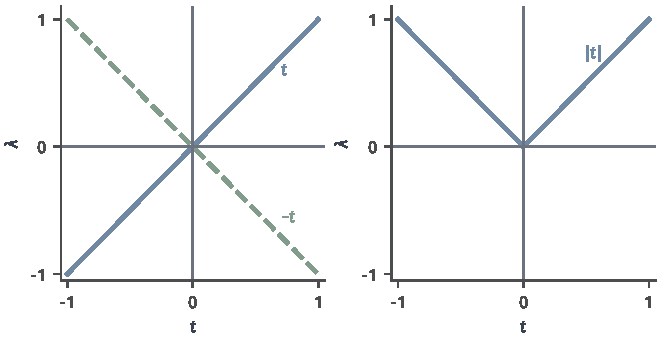
\includegraphics[width=112mm]{figures/02-vectors-matrices-and-multivariate-calculus/04-multivariate-calculus/matplotlib/explanation-additions/ordered-eigenvalue-kink.pdf}
\caption{$\bm S(t)=\operatorname{diag}(t,-t)$。左图为未排序分支$t$与$-t$，右图为最大特征值$|t|$。两侧斜率在零点不同，但函数仍为$1$-Lipschitz，零点的局部绝对条件数仍为$1$。}
\label{fig:v2-ordered-eigenvalue-kink}
\end{figure}

反过来，局部条件数为零也不说明输出不变。$f(t)=t^2$在$0$处导数为零，局部条件数为$0$，但有限步长$t$仍带来变化$t^2$。一阶分析在这里预测“没有变化”，被遗漏的部分要由下一小节的余项界估计。

\subsection{一阶近似的余项界}
\label{sec:multivariable-first-order-remainder}

可微性只保证余项是$o(\lVert\bm h\rVert)$，并不给出某个有限扰动的数值误差界。要得到这样的界，需要知道导数沿扰动线段怎样变化。本小节输入、输出都取欧氏范数，矩阵空间取Frobenius范数，即拉直后的欧氏范数；导数的大小用谱范数度量。其他范数下可借范数等价改变常数。

设$F$在包含线段$[\bm x,\bm x+\bm h]$的开集上连续可微。式~\eqref{eq:multivariable-vector-integral-increment}给出完整增量$\int_0^1\bm J_F(\bm x+t\bm h)\bm h\,\mathrm dt$；从中扣除常向量$\bm J_F(\bm x)\bm h=\int_0^1\bm J_F(\bm x)\bm h\,\mathrm dt$，得到余项的精确表示
\begin{equation}
 R_{\bm x}(\bm h)=F(\bm x+\bm h)-F(\bm x)-\bm J_F(\bm x)\bm h
 =\int_0^1\bigl(\bm J_F(\bm x+t\bm h)-\bm J_F(\bm x)\bigr)\bm h\,\mathrm dt .
\label{eq:multivariable-remainder-integral}
\end{equation}
对照两种估计：完整增量由沿线段的导数大小$\lVert\bm J_F\rVert_2$控制（式~\eqref{eq:analysis-operator-mean-value-bound}），余项则由导数相对基点的变化$\lVert\bm J_F(\bm x+t\bm h)-\bm J_F(\bm x)\rVert_2$控制。导数很大而变化很慢时，整个增量可以很大，一阶预测却仍然准确；二者估计的是不同对象。
\begin{theorem}[一阶近似的二次余项界]
\label{thm:multivariable-first-order-remainder-bound}
设$F$在包含线段$[\bm x,\bm x+\bm h]$的开集上连续可微，且存在常数$L\geq0$，使
\[
 \lVert\bm J_F(\bm y)-\bm J_F(\bm x)\rVert_2\leq L\lVert\bm y-\bm x\rVert_2\qquad(\bm y\in[\bm x,\bm x+\bm h]).
\]
则
\begin{equation}
 \lVert F(\bm x+\bm h)-F(\bm x)-\bm J_F(\bm x)\bm h\rVert_2\leq\frac L2\lVert\bm h\rVert_2^2 .
\label{eq:multivariable-first-order-remainder-bound}
\end{equation}
\end{theorem}
\begin{proof}
取$\bm y=\bm x+t\bm h$，假设给出
\[
 \lVert\bm J_F(\bm x+t\bm h)-\bm J_F(\bm x)\rVert_2\leq Lt\lVert\bm h\rVert_2 .
\]
对式~\eqref{eq:multivariable-remainder-integral}使用向量积分的范数不等式与谱范数的界，
\[
 \lVert R_{\bm x}(\bm h)\rVert_2
 \leq\int_0^1\bigl\lVert\bigl(\bm J_F(\bm x+t\bm h)-\bm J_F(\bm x)\bigr)\bm h\bigr\rVert_2\,\mathrm dt
 \leq\int_0^1Lt\lVert\bm h\rVert_2^2\,\mathrm dt=\frac L2\lVert\bm h\rVert_2^2 .
\]
\end{proof}
定理只要求一阶导数相对基点满足Lipschitz型的界，不以Hessian或二阶导数的存在为前提。若$\bm J_F$在一个凸邻域内以$L$为Lipschitz常数，邻域内每条线段都满足假设。定理~\ref{thm:multivariable-second-derivative-lipschitz}已说明，$F\in C^2$时二阶导数的统一界$M$就是这样的常数，于是余项不超过$M\lVert\bm h\rVert_2^2/2$；这是取得该条件的一种充分办法。

上界正比于$\lVert\bm h\rVert_2^2$：步长缩小到一半，上界缩小到四分之一。这说明的是所保证误差的量级，并不意味着实际误差恰好按同样比例变化，实际误差也可能远小于上界。

例如对称二次型$q(\bm x)=\bm x^\top\bm S\bm x$的Jacobian是$\nabla q^\top=2\bm x^\top\bm S$，满足
\[
 \lVert2\bm S\bm y-2\bm S\bm x\rVert_2\leq2\lVert\bm S\rVert_2\lVert\bm y-\bm x\rVert_2 ;
\]
定理给出余项界$\lVert\bm S\rVert_2\lVert\bm h\rVert_2^2$，与第~\ref{sec:multivariable-differential-rules}节由精确增量得到的$|\bm h^\top\bm S\bm h|\leq\lVert\bm S\rVert_2\lVert\bm h\rVert_2^2$一致。

\paragraph{三种保证的分工}
可微给出统一的$o(\lVert\bm h\rVert)$，只说明步长趋零时的行为；导数的Lipschitz界给出带明确常数的二次余项；第~\ref{sec:multivariable-vector-increment-bound}节的导数界则控制整个有限变化。

使用后两者之前都要先检查：扰动线段是否留在定义域内，可逆、正定等结构条件是否在整条线段上保持，所需常数是否在这个范围内统一成立。矩阵映射的这些检查可以借助已有的有限扰动结论：第~\ref{chap:condition-and-spectral-perturbation}章的Weyl界与奇异值扰动界判断正定性与可逆性是否保持，第~\ref{sec:ls-inverse-sensitivity}节的逆矩阵有限界控制求逆在整段上的变化。基点的条件数只描述无穷小扰动，不能代替这些范围检查和余项估计；下一节对各种矩阵运算逐一完成这些检查。

\section{矩阵运算的扰动分析}
\label{sec:multivariable-matrix-operation-perturbation}

第~\ref{chap:matrix-differentiation}章已经求出常用矩阵运算的微分，并用增量的一阶项验证了可微性。本节回到误差问题：矩阵数据带有扰动$\bm E$时，这些微分给出的线性预测在有限步长下有多准，误差在最坏方向上被放大多少。

对每种运算都要同时检查三件事：输出是矩阵还是标量，因而误差用什么范数或尺度度量；扰动是否受对称等结构限制；整条扰动线段是否留在定义域内。前一节的一般原则在这里落到具体的余项表达式上。本节的矩阵范数除特别说明外取满足乘积不等式$\lVert\bm X\bm Y\rVert\leq\lVert\bm X\rVert\lVert\bm Y\rVert$的范数，例如谱范数或Frobenius范数；求逆时取由向量范数诱导的矩阵范数，它还满足$\lVert\bm I\rVert=1$。

\subsection{基本矩阵运算的增量与余项}
\label{sec:multivariable-basic-operation-remainder}

第~\ref{sec:multivariable-matrix-basic-operations}节对转置、乘法、平方、迹、Frobenius范数平方和二次型写出了精确增量。这些增量都是扰动的多项式，所以余项不必另行估计，直接从增量中读出，再用范数控制大小。

\paragraph{线性运算}
加法、数乘、转置、迹以及$\bm X\mapsto\bm A\bm X\bm B$都是线性映射，精确增量就是一阶项，余项恒为零。对这些运算，线性预测在任意步长下都精确，误差问题只剩放大倍数。由定理~\ref{thm:multivariable-local-condition-number}，局部绝对条件数就是运算本身的算子范数，且与基点无关。

例如在Frobenius范数下，转置不改变任何矩阵的长度，条件数为$1$。迹则不同：由Cauchy--Schwarz不等式，
\[
 |\operatorname{tr}\bm E|=|\langle\bm I,\bm E\rangle_F|\leq\sqrt d\,\lVert\bm E\rVert_F ,
\]
取$\bm E=\bm I/\sqrt d$时等号成立，所以$d\times d$矩阵的迹的条件数为$\sqrt d$。各对角元的误差同号时会累加起来。

\paragraph{乘积与平方}
由式~\eqref{eq:multivariable-product-increment}，两个因子同时扰动时，
\[
 (\bm A+\bm E)(\bm B+\bm H)-\bm A\bm B-(\bm A\bm H+\bm E\bm B)=\bm E\bm H .
\]
由乘积不等式，一阶项与余项分别满足
\[
 \begin{gathered}
 \lVert\bm A\bm H+\bm E\bm B\rVert\leq\lVert\bm A\rVert\lVert\bm H\rVert+\lVert\bm E\rVert\lVert\bm B\rVert,\\
 \lVert\bm E\bm H\rVert\leq\lVert\bm E\rVert\lVert\bm H\rVert .
 \end{gathered}
\]
两者的比较说明：两个扰动都不超过$\rho$时，一阶项至多与$\rho$同阶，余项至多是$\rho^2$。

平方映射同理，$(\bm X+\bm E)^2-\bm X^2$的一阶项为$\bm X\bm E+\bm E\bm X$，余项恰为$\bm E^2$，且$\lVert\bm E^2\rVert\leq\lVert\bm E\rVert^2$。

这些界可以直接用作误差预算。若要求线性预测的绝对误差不超过$\tau$，乘积情形只需$\lVert\bm E\rVert\lVert\bm H\rVert\leq\tau$，两个扰动同样大小时步长不超过$\sqrt\tau$即可。若要求余项不超过一阶项的某个比例，则还要知道一阶项在所取方向上有多大，不能只看扰动的大小。
\begin{example}[矩阵平方的一阶预测]
\label{ex:multivariable-square-first-order-check}
取$\bm X=\operatorname{diag}(2,1)$与扰动$\bm E=\varepsilon\bm K$，其中
\[
 \bm K=\begin{bmatrix}0&1\\1&0\end{bmatrix}.
\]
一阶项与余项分别为
\[
 \bm X\bm E+\bm E\bm X=\varepsilon\begin{bmatrix}0&3\\3&0\end{bmatrix},\qquad
 \bm E^2=\varepsilon^2\bm I ,
\]
谱范数分别为$3\varepsilon$与$\varepsilon^2$。取$\varepsilon=0.1$，一阶项为$0.3$，余项为$0.01$，约为一阶项的$3\%$。

若要求余项不超过一阶项的$1\%$，需要
\[
 \frac{\varepsilon^2}{3\varepsilon}\leq0.01 ,
\]
即扰动须满足$\varepsilon\leq0.03$。
\end{example}

\paragraph{Frobenius范数平方与二次型}
标量输出的运算同样可以读出余项。Frobenius范数平方的精确增量为
\[
 \lVert\bm X+\bm E\rVert_F^2-\lVert\bm X\rVert_F^2=2\langle\bm X,\bm E\rangle_F+\lVert\bm E\rVert_F^2 ,
\]
余项恰为$\lVert\bm E\rVert_F^2$，与方向无关。一阶项$2\langle\bm X,\bm E\rangle_F$却可能为零：扰动与$\bm X$正交时，线性预测说“没有变化”，实际变化却是$\lVert\bm E\rVert_F^2$。这时余项与一阶项之比没有意义，应直接给出绝对误差的预算。

二次型$\bm x^\top\bm A\bm x$在$\bm A$与$\bm x$同时扰动时，第~\ref{sec:multivariable-matrix-basic-operations}节写出的余项为
\[
 \bm h^\top\bm A\bm h+\bm x^\top\bm E\bm h+\bm h^\top\bm E\bm x+\bm h^\top\bm E\bm h .
\]
在谱范数下，它的绝对值不超过
\[
 \lVert\bm A\rVert_2\lVert\bm h\rVert_2^2+2\lVert\bm E\rVert_2\lVert\bm x\rVert_2\lVert\bm h\rVert_2+\lVert\bm E\rVert_2\lVert\bm h\rVert_2^2 .
\]
每一项都含两个扰动因子，其中$\lVert\bm E\rVert_2\lVert\bm h\rVert_2$一项还乘了基点的大小$\lVert\bm x\rVert_2$：基点越大，矩阵与向量扰动的交叉作用越强。

比较起来，线性运算的余项为零，多项式运算的余项是扰动的二次或更高次项，并且可以精确写出。误差预算由这些高次项决定线性预测可用的步长；导数本身的大小只决定一阶项，不决定预测还差多少。

\subsection{求逆的扰动}
\label{sec:multivariable-inverse-perturbation}

第~\ref{sec:multivariable-inverse-differential}节由逆差恒等式证明了求逆可微，并得到$\mathrm d(\bm X^{-1})=-\bm X^{-1}\mathrm d\bm X\bm X^{-1}$。那里只用到余项是$o(\lVert\bm E\rVert)$。本节把余项精确写出，给出它的二次界，再计算求逆的条件数，并说明它与线性方程解映射的联系。

\paragraph{精确余项与可逆邻域}
设$\bm A$可逆，$\bm B=\bm A+\bm E$，$q=\lVert\bm A^{-1}\rVert\lVert\bm E\rVert<1$。由逆差恒等式~\eqref{eq:ch06-inverse-finite-perturbation}，
\[
 \bm B^{-1}-\bm A^{-1}=-\bm B^{-1}\bm E\bm A^{-1}.
\]
把右端的$\bm B^{-1}$写成$\bm A^{-1}+(\bm B^{-1}-\bm A^{-1})$，再用一次同一恒等式，
\[
 \bm B^{-1}-\bm A^{-1}
 =-\bm A^{-1}\bm E\bm A^{-1}-(\bm B^{-1}-\bm A^{-1})\bm E\bm A^{-1}
 =-\bm A^{-1}\bm E\bm A^{-1}+\bm B^{-1}\bm E\bm A^{-1}\bm E\bm A^{-1}.
\]
第一项是一阶预测，第二项是精确余项。由$\lVert\bm B^{-1}\rVert\leq\lVert\bm A^{-1}\rVert/(1-q)$（第~\ref{sec:ls-inverse-sensitivity}节），
\begin{equation}
 \lVert\bm B^{-1}\bm E\bm A^{-1}\bm E\bm A^{-1}\rVert
 \leq\lVert\bm B^{-1}\rVert\lVert\bm A^{-1}\rVert^2\lVert\bm E\rVert^2
 \leq\frac{\lVert\bm A^{-1}\rVert^3\lVert\bm E\rVert^2}{1-q}.
\label{eq:multivariable-inverse-remainder-bound}
\end{equation}

第~\ref{chap:linear-recurrence-stability}章的Neumann级数给出同一结论的另一种看法。写$\bm B=\bm A(\bm I-\bm T)$，其中$\bm T=-\bm A^{-1}\bm E$，$\lVert\bm T\rVert\leq q<1$，因而谱半径小于$1$。由定理~\ref{thm:ls-neumann}，$\bm I-\bm T$可逆，且
\[
 \bm B^{-1}=\sum_{k\geq0}\bm T^k\bm A^{-1}.
\]
前两项$\bm A^{-1}-\bm A^{-1}\bm E\bm A^{-1}$正是一阶预测；截断误差界~\eqref{eq:ls-neumann-tail}取$N=1$，给出余项不超过$q^2\lVert\bm A^{-1}\rVert/(1-q)$，与式~\eqref{eq:multivariable-inverse-remainder-bound}相同。级数还说明，余项依次由$\bm E$的二次、三次……项组成。

\paragraph{一阶预测的误差}
式~\eqref{eq:multivariable-inverse-remainder-bound}同时是有限扰动下一阶预测的误差界。对$0\leq t\leq1$，$\lVert\bm A^{-1}(t\bm E)\rVert\leq tq<1$，所以整条扰动线段$\bm A+t\bm E$都由可逆矩阵组成，定义域条件在整段上成立。

于是可以比较三个量：实际逆矩阵$(\bm A+\bm E)^{-1}$，一阶预测$\bm A^{-1}-\bm A^{-1}\bm E\bm A^{-1}$，以及二者之差。第~\ref{sec:ls-inverse-sensitivity}节控制的是全变化，
\[
 \lVert(\bm A+\bm E)^{-1}-\bm A^{-1}\rVert\leq\frac{\lVert\bm A^{-1}\rVert^2\lVert\bm E\rVert}{1-q},
\]
与$\lVert\bm E\rVert$同阶；本段新增的是从全变化中扣除一阶项之后，近似还差多少，它与$\lVert\bm E\rVert^2$同阶。$q$接近$1$时两种界都变得很大，一阶预测不再可靠。
\begin{example}[逆矩阵的一阶预测与余项]
\label{ex:multivariable-inverse-first-order-check}
取$\bm A=\operatorname{diag}(2,1)$与扰动
\[
 \bm E=\begin{bmatrix}0&0.1\\0.1&0\end{bmatrix},
\]
采用谱范数，则$\lVert\bm A^{-1}\rVert_2=1$、$\lVert\bm E\rVert_2=0.1$、$q=0.1$。这个矩阵可以直接求逆，
\[
 (\bm A+\bm E)^{-1}=\frac1{1.99}\begin{bmatrix}1&-0.1\\-0.1&2\end{bmatrix},
\]
而一阶预测为
\[
 \bm A^{-1}-\bm A^{-1}\bm E\bm A^{-1}=\begin{bmatrix}0.5&-0.05\\-0.05&1\end{bmatrix}.
\]
实际值减去预测，剩下的余项为
\[
 \frac{0.0005}{1.99}\begin{bmatrix}10&-1\\-1&20\end{bmatrix}\approx\begin{bmatrix}0.00251&-0.00025\\-0.00025&0.00503\end{bmatrix}.
\]

现在比较几个量的大小。余项的谱范数约为$0.00505$，约为一阶项谱范数$0.05$的十分之一，并落在式~\eqref{eq:multivariable-inverse-remainder-bound}的上界$0.01/0.9\approx0.0111$之内。

再看全变化。全变化$(\bm A+\bm E)^{-1}-\bm A^{-1}$的谱范数约为$0.0540$，第~\ref{sec:ls-inverse-sensitivity}节的全变化界为$0.1/0.9\approx0.111$。
\end{example}
一阶预测扣除了全变化中约$0.05$的主要部分，剩下的误差约为扰动大小的平方量级；余项界比实际误差大约两倍，它只保证误差不超过多少。

\paragraph{求逆的条件数}
在无结构限制的扰动模型下，输入、输出都取谱范数。由乘积不等式，
\[
 \lVert\bm A^{-1}\bm E\bm A^{-1}\rVert_2\leq\lVert\bm A^{-1}\rVert_2^2\lVert\bm E\rVert_2 .
\]

这个上界可以取到。设$\sigma_d$是$\bm A$的最小奇异值，对应的左、右奇异向量为$\bm u_d,\bm v_d$，即$\bm A\bm v_d=\sigma_d\bm u_d$、$\bm A^\top\bm u_d=\sigma_d\bm v_d$（第~\ref{sec:ls-svd}章）。取$\bm E=\bm u_d\bm v_d^\top$，它的谱范数为$1$。由$\bm A^{-1}\bm u_d=\bm v_d/\sigma_d$与$\bm A^{-\top}\bm v_d=\bm u_d/\sigma_d$，
\[
 \bm A^{-1}\bm E\bm A^{-1}=(\bm A^{-1}\bm u_d)(\bm A^{-\top}\bm v_d)^\top=\frac{\bm v_d\bm u_d^\top}{\sigma_d^2},
\]
其谱范数为$1/\sigma_d^2=\lVert\bm A^{-1}\rVert_2^2$。

由定理~\ref{thm:multivariable-local-condition-number}，求逆映射在$\bm A$处的局部绝对条件数为$\lVert\bm A^{-1}\rVert_2^2$，相对条件数为
\[
 \lVert\bm A^{-1}\rVert_2^2\cdot\frac{\lVert\bm A\rVert_2}{\lVert\bm A^{-1}\rVert_2}=\lVert\bm A\rVert_2\lVert\bm A^{-1}\rVert_2=\kappa_2(\bm A).
\]

矩阵条件数在这里重新出现，但含义不同：这里输入是矩阵本身，输出是逆矩阵，而第~\ref{sec:ls-matrix-condition-number}节的输入是向量。若限制扰动结构，例如只允许对称扰动，须改用微分在允许子空间上的范数。求解方程的算法及其数值稳定性仍按第~\ref{chap:solution-error-regularization}章处理。

\paragraph{线性方程的解映射}
求逆与乘法复合，得到线性方程的解映射
\[
 \operatorname{sol}(\bm A,\bm b)=\bm A^{-1}\bm b ,
\]
它定义在可逆$\bm A$与任意$\bm b$组成的开集上。固定可逆的$\bm A$，记$\bm x=\bm A^{-1}\bm b$；联合输入$(\bm E,\bm f)$取乘积范数$\lVert(\bm E,\bm f)\rVert=(\lVert\bm E\rVert^2+\lVert\bm f\rVert^2)^{1/2}$，其中$\bm f$是右端的增量。

第~\ref{sec:ls-equation-sensitivity}节从扰动后的方程
\[
 (\bm A+\bm E)(\bm x+\Delta\bm x)=\bm b+\bm f
\]
中减去$\bm A\bm x=\bm b$，得到
\[
 (\bm A+\bm E)\Delta\bm x=\bm f-\bm E\bm x .
\]
在$q<1$时，这给出精确式
\[
 \Delta\bm x=(\bm A+\bm E)^{-1}(\bm f-\bm E\bm x).
\]
把$(\bm A+\bm E)^{-1}$拆成$\bm A^{-1}$与逆差，
\[
 \Delta\bm x=\bm A^{-1}(\bm f-\bm E\bm x)+\bigl((\bm A+\bm E)^{-1}-\bm A^{-1}\bigr)(\bm f-\bm E\bm x).
\]
第一项对$(\bm E,\bm f)$线性。第二项中，两个因子分别满足
\[
 \begin{gathered}
 \bigl\lVert(\bm A+\bm E)^{-1}-\bm A^{-1}\bigr\rVert\leq\frac{\lVert\bm A^{-1}\rVert^2\lVert\bm E\rVert}{1-q},\\
 \lVert\bm f-\bm E\bm x\rVert\leq\lVert\bm f\rVert+\lVert\bm E\rVert\lVert\bm x\rVert ;
 \end{gathered}
\]
二者都不超过联合扰动大小的常数倍，所以第二项是联合扰动的二次量。因此解映射可微，且
\begin{equation}
 \mathrm d\operatorname{sol}_{(\bm A,\bm b)}(\bm E,\bm f)=\bm A^{-1}(\bm f-\bm E\bm x).
\label{eq:multivariable-solution-map-differential}
\end{equation}
也可以用链式法则核对：$\operatorname{sol}$是求逆与矩阵—向量乘法的复合，由乘积的联合微分与式~\eqref{eq:analysis-inverse-differential}，一阶项为
\[
 (-\bm A^{-1}\bm E\bm A^{-1})\bm b+\bm A^{-1}\bm f=\bm A^{-1}(\bm f-\bm E\bm x),
\]
结果相同。第~\ref{sec:multivariable-implicit-function}节已用隐函数公式核对过同一结果。

第~\ref{sec:ls-equation-sensitivity}节的界控制完整的解误差，式~\eqref{eq:multivariable-solution-map-differential}则提取局部的一阶预测，上面的拆分还说明预测的误差是联合扰动的二次量。数据误差、残差与算法稳定性的完整分析仍以第~\ref{chap:solution-error-regularization}章为准，本节只补充一阶响应及其精度。

\subsection{行列式的扰动}
\label{sec:multivariable-determinant-perturbation}

第~\ref{sec:multivariable-determinant-differential}节逐列展开$\det(\bm A+\bm E)$，得到一阶项$\langle\bm C,\bm E\rangle_F$，其中$\bm C$是代数余子式矩阵；展开中其余各项至少含两列扰动。这些高阶项就是线性预测的误差。它们对包括奇异矩阵在内的全部方阵都有意义，所以先讨论绝对误差，再在可逆时讨论相对误差。

\paragraph{绝对变化的余项}
在固定的有界邻域内，余项有二次控制。记$K=\{\bm A+\bm F:\lVert\bm F\rVert_F\leq1\}$。行列式的二阶偏导数都是多项式，在闭有界集$K$上有界，所以存在$M$使$\lVert D^2\det_{\bm Z}\rVert\leq M$对$\bm Z\in K$成立。

对$\lVert\bm E\rVert_F\leq1$，令$g(t)=\det(\bm A+t\bm E)$，它是$t$的多项式。它的二阶导数及其界为
\[
 g''(t)=D^2\det_{\bm A+t\bm E}[\bm E,\bm E],\qquad |g''(t)|\leq M\lVert\bm E\rVert_F^2 .
\]
一元Taylor公式给出
\[
 \bigl|\det(\bm A+\bm E)-\det\bm A-\langle\bm C,\bm E\rangle_F\bigr|\leq\frac M2\lVert\bm E\rVert_F^2 ,
\]
常数$M$依赖所取的邻域。

二阶情形可以精确写出余项。对$\bm A,\bm E\in\mathbb R^{2\times2}$，直接展开得
\[
 \det(\bm A+\bm E)=\det\bm A+\langle\bm C,\bm E\rangle_F+\det\bm E ,
\]
余项就是$\det\bm E=E_{1,1}E_{2,2}-E_{1,2}E_{2,1}$。由$|ab|\leq(a^2+b^2)/2$，
\[
 |\det\bm E|\leq\frac{\lVert\bm E\rVert_F^2}2 ,
\]
即上式中可取$M=1$，而且这个界与基点$\bm A$无关，奇异的$\bm A$也适用。

\paragraph{条件数与相对变化}
对给定扰动方向，一阶响应是$\langle\bm C,\bm E\rangle_F$。由定理~\ref{thm:multivariable-local-condition-number}，局部绝对条件数是这个线性泛函在所选输入范数下的大小，即第~\ref{sec:ls-dual-norms}节的对偶范数：
\[
 \kappa_{\mathrm{abs}}(\det,\bm A)=\max_{\lVert\bm E\rVert\leq1}|\langle\bm C,\bm E\rangle_F| .
\]
输入取Frobenius范数时，由Cauchy--Schwarz不等式，$\bm C\neq\bm0$时最大值在$\bm E=\bm C/\lVert\bm C\rVert_F$处取到，所以$\kappa_{\mathrm{abs}}=\lVert\bm C\rVert_F$，可以直接由代数余子式算出。

可逆时还可以比较相对变化：由$\bm C=\det(\bm A)\bm A^{-\top}$，
\[
 \kappa_{\mathrm{rel}}(\det,\bm A)=\lVert\bm C\rVert_F\frac{\lVert\bm A\rVert_F}{|\det\bm A|}=\lVert\bm A^{-1}\rVert_F\lVert\bm A\rVert_F .
\]
奇异点处$\det\bm A=0$，只有绝对变化有定义，不能除以零行列式。

在相对尺度下，行列式对矩阵变化的反应可以远比矩阵本身的变化剧烈。
\begin{example}[接近奇异时的行列式]
\label{ex:ls-determinant-near-singular}
设$\bm A=\operatorname{diag}(1,\varepsilon)$，$0<\varepsilon<1$，它的行列式$\det\bm A=\varepsilon$很小。只改动第二个对角元，取扰动$\bm E=\operatorname{diag}(0,\delta)$，使它变为$\varepsilon+\delta$。矩阵采用谱范数、标量采用绝对值时，矩阵的相对变化为$\lVert\bm E\rVert_2/\lVert\bm A\rVert_2=|\delta|$；行列式则变为$\varepsilon+\delta$，相对变化为
\[
 \frac{|(\varepsilon+\delta)-\varepsilon|}{\varepsilon}=\frac{|\delta|}{\varepsilon}.
\]
用微分公式计算也得到同样的增量：
\[
 \det(\bm A)\operatorname{tr}(\bm A^{-1}\bm E)=\varepsilon\cdot\frac\delta\varepsilon=\delta .
\]
沿这个方向，行列式是$\delta$的一次函数，所以一阶预测没有余项。

两相比较，行列式的相对变化是矩阵相对变化的$1/\varepsilon$倍。$\varepsilon$越小，矩阵越接近奇异，沿这个方向的相对放大就越强。
\end{example}

但不能仅凭行列式的数值判断求逆是否病态。取$\bm A=\varepsilon\bm I\in\mathbb R^{d\times d}$（$\varepsilon>0$），行列式$\varepsilon^d$可以极小，而由第~\ref{sec:multivariable-inverse-perturbation}节，求逆的相对条件数是$\kappa_2(\varepsilon\bm I)=1$；行列式本身的相对条件数$\lVert\bm A^{-1}\rVert_F\lVert\bm A\rVert_F=d$也不随$\varepsilon$变大。行列式与逆矩阵是两个不同的输出，绝对与相对又是两种尺度，必须分别判断。

\subsection{对数行列式的扰动}
\label{sec:multivariable-logdet-perturbation}

由第~\ref{sec:multivariable-logdet-differential}节，$\log\det$在$\det>0$的开集上可微，微分为$\bm E\mapsto\operatorname{tr}(\bm A^{-1}\bm E)$。它给出一阶变化：
\[
 \log\det(\bm A+\bm E)-\log\det\bm A
 =\operatorname{tr}(\bm A^{-1}\bm E)+o(\lVert\bm E\rVert_F).
\]
相应的局部绝对条件数是线性泛函$\bm E\mapsto\langle\bm A^{-\top},\bm E\rangle_F$在所选输入范数下的对偶范数，Frobenius范数下为$\lVert\bm A^{-1}\rVert_F$。对数行列式可以为零或接近零，这时以它为分母的相对误差没有意义，应直接比较绝对变化。

\paragraph{整条线段的定义域}
要把一阶预测用于有限扰动，先要保证整条线段$\bm A+t\bm E$（$0\leq t\leq1$）留在定义域内。一般的正行列式矩阵，由行列式的连续性，总可以选足够小的邻域，使整条线段$\bm A+t\bm E$仍满足$\det>0$，但这不给出邻域的具体大小。正定情形则可以用第~\ref{chap:condition-and-spectral-perturbation}章的最小特征值界明确检查整条线段保持正定，下面的余项界就基于这一检查。

\paragraph{二次余项界}
设$\bm A$对称正定，最小特征值为$m>0$，$\bm E$对称且$\lVert\bm E\rVert_2<m$。对任意单位向量$\bm x$和$0\leq t\leq1$，
\[
 \bm x^\top(\bm A+t\bm E)\bm x\geq m-\lVert\bm E\rVert_2>0 ,
\]
所以整条线段保持正定，而且最小特征值有统一的正下界。

令$g(t)=\log\det(\bm A+t\bm E)$。由式~\eqref{eq:analysis-logdet-gradient}与链式法则，
\[
 g'(t)=\operatorname{tr}\bigl((\bm A+t\bm E)^{-1}\bm E\bigr);
\]
再用沿参数曲线的求逆公式，
\[
 g''(t)=-\operatorname{tr}\!\left((\bm A+t\bm E)^{-1}\bm E
 (\bm A+t\bm E)^{-1}\bm E\right).
\]
逆矩阵的谱范数至多为$(m-\lVert\bm E\rVert_2)^{-1}$。由Frobenius内积的Cauchy--Schwarz不等式与混合乘积界~\eqref{eq:matrix-analysis-mixed-submultiplicativity}，
\[
 |g''(t)|\leq\lVert(\bm A+t\bm E)^{-1}\bm E\rVert_F^2\leq\frac{\lVert\bm E\rVert_F^2}{(m-\lVert\bm E\rVert_2)^2}.
\]
于是一元Taylor公式给出
\begin{equation}
 \left|\log\det(\bm A+\bm E)-\log\det\bm A
 -\operatorname{tr}(\bm A^{-1}\bm E)\right|
 \leq\frac{\lVert\bm E\rVert_F^2}{2(m-\lVert\bm E\rVert_2)^2}.
\label{eq:multivariable-logdet-remainder-bound}
\end{equation}

例如$\bm A=\operatorname{diag}(2,1)$，$\bm E=\operatorname{diag}(0.1,0)$时，一阶预测为$0.05$，实际变化为$\log(1.05)\approx0.04879$。此时$m=1$，上述上界约为$0.00618$，大于实际误差约$0.00121$。这个界只保证误差不超过多少，不表示误差会接近上界。

导数给出变化的方向与大小，正定线段给出估计的有效范围，余项界说明预测的可靠程度，三者要一起使用。正定条件是这一显式估计的条件，不是一般正行列式矩阵上$\log\det$的定义条件。

上界的分母$m-\lVert\bm E\rVert_2$是扰动后最小特征值的保底下界，即到奇异边界的余量。$\bm A$接近奇异时，$m$很小：一阶响应的条件数$\lVert\bm A^{-1}\rVert_F\geq1/m$变大，余项界又按$1/(m-\lVert\bm E\rVert_2)^2$放大，允许的步长必须小于$m$。

例如$\bm A=\operatorname{diag}(1,\varepsilon)$、$\bm E=\operatorname{diag}(0,\delta)$时，精确变化是$\log(1+\delta/\varepsilon)$，一阶预测是$\delta/\varepsilon$；$\delta$与$\varepsilon$同阶时两者相差显著，$\delta\to-\varepsilon$时精确值趋于$-\infty$。

\section{特征值与特征向量的微分}
\label{sec:multivariable-eigen-differential}

特征值和特征向量由方程$\bm S\bm v=\lambda\bm v$确定，并不是矩阵元素的显式函数，前一节的显式计算不能直接使用。第~\ref{chap:condition-and-spectral-perturbation}章已经给出有限扰动下的稳定性界：对称扰动$\bm E$使每个排序后的特征值至多移动$\lVert\bm E\rVert_2$（Weyl界，定理~\ref{thm:ls-weyl-eigenvalue}），特征子空间的偏转受$\lVert\bm E\rVert_2$与谱隙之比控制（第~\ref{sec:ls-subspace-sensitivity}节）。这些界对一切方向取最坏情形。

本节回答另一个问题：沿一个指定的扰动方向，特征值与特征向量以什么速率变化，这个变化率在多大范围内可以用来预测。先用第~\ref{chap:implicit-inverse-functions}章的隐函数定理证明简单特征值所在的分支可微，再分别计算特征值与特征向量的微分，最后说明一阶近似的适用条件。

\subsection{特征值与特征向量的可微性}
\label{sec:multivariable-eigen-differentiability}

设实对称矩阵$\bm S_0\in\mathbb R^{d\times d}$有一个简单特征值$\lambda_0$，对应单位特征向量$\bm v_0$。简单是指这个特征值的代数重数为$1$；对实对称矩阵，这等价于其特征空间是一维的。即使规定长度为$1$，$\bm v_0$和$-\bm v_0$仍代表同一方向。为了在局部选定一支，我们要求附近的向量$\bm v$满足$\bm v_0^\top\bm v>0$。这里选出的只是一个局部分支，单位长度本身并不保证全局唯一。

把对称矩阵$\bm S$作为参数，选取其上三角元素作为独立坐标，便可把对称矩阵空间视为有限维欧氏空间。把向量$\bm v$和标量$\lambda$作为未知量，特征方程与单位长度条件合起来写成
\[
 F(\bm S,\bm v,\lambda)=
 \begin{pmatrix}\bm S\bm v-\lambda\bm v\\ (\bm v^\top\bm v-1)/2\end{pmatrix}=\bm0.
\]
这是$d+1$个方程、$d+1$个未知量。在$(\bm S_0,\bm v_0,\lambda_0)$处，关于$(\bm v,\lambda)$的导数作用于$(\bm h,\eta)$，其矩阵为
\[
 \begin{pmatrix}\bm S_0-\lambda_0\bm I&-\bm v_0\\
 \bm v_0^\top&0\end{pmatrix}.
\]
要用隐函数定理，需验证这个方阵可逆，即它只把零向量映为零。设它把$(\bm h,\eta)$映为零，即
\[
 (\bm S_0-\lambda_0\bm I)\bm h-\eta\bm v_0=\bm0,\qquad \bm v_0^\top\bm h=0 .
\]
先用$\bm v_0^\top$左乘第一式，利用对称性及$\bm S_0\bm v_0=\lambda_0\bm v_0$，左端第一项为零，得到$\eta=0$。于是$(\bm S_0-\lambda_0\bm I)\bm h=\bm0$，再由第二式，$\bm h$既属于$\lambda_0$的特征空间，又与$\bm v_0$正交。由于特征值简单，只能有$\bm h=\bm0$。

因此这个方阵可逆，隐函数定理保证在$\bm S_0$附近存在可微的特征值和单位特征向量分支；上述内积为正的条件固定了局部符号。

这里固定符号的条件不能省略。若不选定符号，同一个特征方向可以由$\bm v_0$或$-\bm v_0$表示，沿扰动路径任意切换符号会让“特征向量”看起来不连续；这种跳跃来自表示的不唯一，而不是特征方向本身的变化。选定$\bm v_0^\top\bm v>0$以后，隐函数定理给出的分支在邻域内唯一，可微性才有确定的含义。

\subsection{特征值的微分}
\label{sec:multivariable-eigenvalue-differential}

有了可微分支，就可以求它对每个小的对称扰动方向的一阶响应。设对称扰动方向$\bm E$使特征值与特征向量分别产生一阶变化$\mathrm d\lambda(\bm E)$和$\mathrm d\bm v(\bm E)$。对特征方程与归一化条件求微分，并在基点取值，得到
\begin{equation}
 \begin{gathered}
(\bm S_0-\lambda_0\bm I)\,\mathrm d\bm v(\bm E)
 =-\bigl(\bm E-\mathrm d\lambda(\bm E)\bm I\bigr)\bm v_0,\\
\bm v_0^\top\mathrm d\bm v(\bm E)=0.
 \end{gathered}
 \label{eq:multivariable-eigen-differential-system}
\end{equation}
用$\bm v_0^\top$左乘第一式，左侧为零，于是
\begin{equation}
 \mathrm d\lambda(\bm E)=\bm v_0^\top\bm E\bm v_0.
\label{eq:multivariable-eigenvalue-differential}
\end{equation}
这里的微分作用于全部小的对称方向；可微分支的存在由上一小节的隐函数定理保证，对特征方程形式求导本身不能承担这一步。

公式说明，特征值的变化率只看扰动在该特征方向上的读数$\bm v_0^\top\bm E\bm v_0$。由$\lVert\bm v_0\rVert_2=1$与谱范数的定义，
\[
 |\mathrm d\lambda(\bm E)|=|\bm v_0^\top\bm E\bm v_0|\leq\lVert\bm E\rVert_2 ,
\]
等号在$\bm E=\bm v_0\bm v_0^\top$时取到，所以简单特征值分支的局部绝对条件数（谱范数下）为$1$。与扰动方向正交的部分，例如满足$\bm E\bm v_0=\bm0$的扰动，一阶上不改变这个特征值。
\begin{example}[特征值沿两个方向的变化]
\label{ex:multivariable-eigenvalue-direction-check}
取$\bm S_0=\operatorname{diag}(2,1)$，简单特征值$\lambda_0=2$，$\bm v_0=\bm e_1$。先沿$\bm E_1=\bm e_1\bm e_1^\top$扰动，此时$\bm S_0+t\bm E_1=\operatorname{diag}(2+t,1)$，特征值为$2+t$，变化率为
\[
 1=\bm e_1^\top\bm E_1\bm e_1 ,
\]
余项为零。

再沿下面的方向扰动：
\[
 \bm E_2=\begin{bmatrix}0&1\\1&0\end{bmatrix}.
\]
公式给出$\mathrm d\lambda(\bm E_2)=\bm e_1^\top\bm E_2\bm e_1=0$。直接计算，$\bm S_0+t\bm E_2$的较大特征值为
\[
 \lambda(t)=\frac{3+\sqrt{1+4t^2}}2=2+t^2+O(t^4),
\]
变化确实是二阶的。

两个方向的谱范数都是$1$，Weyl界对两者都只给出$|\lambda(t)-2|\leq|t|$。
\end{example}

例子显示了两类结论的分工。Weyl界是对一切方向、任意步长都成立的最坏偏差；微分是指定方向上的变化率，它可以远小于最坏情形，甚至为零，但只在步长足够小时描述实际变化。用变化率预测有限扰动，还要知道余项多大，这正是最后一小节讨论的问题。

\subsection{特征向量的微分}
\label{sec:multivariable-eigenvector-differential}

特征向量的一阶变化由同一组方程~\eqref{eq:multivariable-eigen-differential-system}确定。把式~\eqref{eq:multivariable-eigenvalue-differential}给出的$\mathrm d\lambda(\bm E)$代回其中的第一式后，第一式右侧与$\bm v_0$正交。由于$\lambda_0$简单，$\bm S_0-\lambda_0\bm I$限制在$\bm v_0$的正交补上可逆，因此第二式选出了唯一的$\mathrm d\bm v(\bm E)$。

\paragraph{谱展开与谱隙}
在$\bm S_0$的标准正交特征基中，向量响应可以显式写出。设$\bm S_0\bm v_j=\lambda_j\bm v_j$（$j=1,\ldots,d$），$\bm v_1,\ldots,\bm v_d$标准正交，并记$\bm v_0=\bm v_i$、$\lambda_0=\lambda_i$。$\mathrm d\bm v(\bm E)$与$\bm v_i$正交，可写成$\sum_{j\neq i}c_j\bm v_j$。代入第一式，左侧为
\[
 (\bm S_0-\lambda_i\bm I)\sum_{j\neq i}c_j\bm v_j=\sum_{j\neq i}c_j(\lambda_j-\lambda_i)\bm v_j ;
\]
与$\bm v_j$（$j\neq i$）作内积，右侧给出$-\bm v_j^\top\bm E\bm v_i$，所以
\begin{equation}
 \mathrm d\bm v(\bm E)=\sum_{j\neq i}\frac{\bm v_j^\top\bm E\bm v_i}{\lambda_i-\lambda_j}\,\bm v_j .
\label{eq:multivariable-eigenvector-differential}
\end{equation}
设$d\geq2$，令谱隙$\gamma=\min_{j\neq i}|\lambda_i-\lambda_j|$，它因特征值简单而为正。由标准正交展开的Parseval等式，
\[
 \lVert\mathrm d\bm v(\bm E)\rVert_2^2=\sum_{j\neq i}\frac{(\bm v_j^\top\bm E\bm v_i)^2}{(\lambda_i-\lambda_j)^2}
 \leq\frac1{\gamma^2}\sum_{j}(\bm v_j^\top\bm E\bm v_i)^2=\frac{\lVert\bm E\bm v_i\rVert_2^2}{\gamma^2}\leq\frac{\lVert\bm E\rVert_2^2}{\gamma^2},
\]
即$\lVert\mathrm d\bm v(\bm E)\rVert_2\leq\lVert\bm E\rVert_2/\gamma$。$d=1$时单位特征向量分支恒为$\bm v_0$，微分为零。

特征值的导数界$|\mathrm d\lambda(\bm E)|\leq\lVert\bm E\rVert_2$与这里的特征向量导数界可以一起与第~\ref{sec:ls-spectral-value-sensitivity}节和第~\ref{sec:ls-subspace-sensitivity}节比较。Weyl界与谱隙界控制的是有限扰动下特征值和特征子空间的整体变化；这里给出的是带方向的一阶响应。特征值的响应$\bm v_i^\top\bm E\bm v_i$只看扰动在该特征方向上的读数；特征向量的响应以$\lambda_i-\lambda_j$为分母，说明谱隙小时，扰动可以把特征向量大幅地转向相邻的特征方向。
\begin{example}[特征向量的转向与谱隙]
\label{ex:multivariable-eigenvector-gap-check}
延续示例~\ref{ex:multivariable-eigenvalue-direction-check}，沿$\bm E_2$，公式给出
\[
 \mathrm d\bm v(\bm E_2)=\frac{\bm e_2^\top\bm E_2\bm e_1}{2-1}\bm e_2=\bm e_2 ,
\]
即$\bm v(t)\approx\bm e_1+t\bm e_2$。直接计算，较大特征值的特征向量与$(1,(\lambda(t)-2)/t)^\top$同向，而$(\lambda(t)-2)/t=t+O(t^3)$，与一阶预测一致。

把基点换成$\bm S_0=\operatorname{diag}(1+\gamma,1)$（$\gamma>0$），同一方向的响应变为$\mathrm d\bm v(\bm E_2)=\bm e_2/\gamma$：谱隙缩小为原来的几分之一，特征向量的转向速率就放大几倍。
\end{example}

微分给出的是指定方向上的转向速率，有限扰动下子空间之间的角度、投影距离和偏转界仍以第~\ref{chap:condition-and-spectral-perturbation}章为准：定理~\ref{thm:ls-davis-kahan}给出$\sin\theta\leq\lVert\bm E\rVert_2/\gamma$型的界，其中谱隙按该定理的规定在原矩阵与扰动后矩阵的相应特征值之间度量。导数界$\lVert\bm E\rVert_2/\gamma$与这个有限界形式相同，说明谱隙同时控制无穷小转向和有限偏转。

\subsection{一阶近似的适用条件}
\label{sec:multivariable-eigen-first-order-validity}

前两小节的公式只在简单特征值附近成立，而且只描述步长趋零时的行为。用它们预测有限扰动，需要扰动相对谱隙足够小。示例~\ref{ex:multivariable-eigenvector-gap-check}的第二个基点可以精确算出这一点。

这时扰动后的矩阵为
\[
 \bm S_0+t\bm E_2=\begin{bmatrix}1+\gamma&t\\t&1\end{bmatrix}.
\]
它的较大特征值的特征向量与$\bm e_1$的夹角$\theta$满足
\[
 \tan2\theta=\frac{2t}\gamma ,
\]
一阶预测则是$\theta\approx t/\gamma$。二者在$|t|\ll\gamma$时一致。

$|t|$与$\gamma$同阶时，实际角度明显小于预测，例如$t=\gamma/2$时$\theta=\pi/8\approx0.39$，预测为$0.5$。固定$t$而令$\gamma\to0$时，实际角度趋于$\pi/4$，预测却趋于无穷。

特征值也有同样的现象。较大特征值及其在$|t|\ll\gamma$时的近似为
\[
 1+\frac\gamma2+\sqrt{\frac{\gamma^2}4+t^2}\approx1+\gamma+\frac{t^2}\gamma ;
\]
一阶项为零，二阶项的系数$1/\gamma$随谱隙缩小而增大。所以一阶预测可靠的条件不是“扰动小”，而是“扰动相对谱隙小”。

上面的结论依赖所选特征值简单。重特征值使关于未知量的导数不可逆，因此不能直接沿用这个构造；但这只说明这条论证失效，并不断言每一条特征值分支都不可微，也不意味着矩阵多项式或可逆点处的求逆映射失去光滑性。

第~\ref{sec:multivariable-local-condition-number}节的$\operatorname{diag}(t,-t)$说明，在重特征值处，排序后的特征值可以有有限条件数而不可微，未排序的分支却仍然光滑。研究重特征值附近时，应改为考察相应的特征子空间，而不是强行指定其中某一个特征向量；谱簇子空间的稳定性已在第~\ref{sec:ls-subspace-sensitivity}节处理，这里不重复谱扰动界。

总之，本节只界定简单谱分支何时可微，以及微分公式何时可以用作一阶近似。重根附近的稳定性需要把相邻特征值合成隔离的特征簇，比较整个特征子空间；这部分直接使用第~\ref{chap:condition-and-spectral-perturbation}章的结论。

\FloatBarrier
\section{本章小结}
\label{sec:differential-perturbation-summary}

本章用三个量回答输入扰动的影响。微分给出指定方向上的一阶响应$\mathrm dF_{\bm x}(\bm h)$；局部条件数是这些响应在全部允许方向上的最坏放大倍数，可微时等于微分在允许方向子空间上的算子范数；余项说明给定步长下线性预测还差多少。三者回答不同的问题：条件数只描述无穷小扰动，可以有限而映射不可微，也可以为零而有限变化不为零；余项界需要导数沿整条扰动线段的Lipschitz型控制，二阶导数的统一界是取得这一控制的充分办法。

显式矩阵运算与隐式谱分支遵循同一套步骤：确定输出类型与误差尺度，限定允许的扰动结构，检查整条线段留在定义域内，再由微分读出响应与条件数、由精确增量或二阶信息估计余项。

线性运算的余项为零；乘积、平方与二次型的余项是可以精确写出的高次项；求逆的余项由逆差恒等式或Neumann级数给出，界为$\lVert\bm A^{-1}\rVert^3\lVert\bm E\rVert^2/(1-q)$，相对条件数是$\kappa_2(\bm A)$；行列式的绝对变化在奇异处也有二次余项控制，相对条件数只在可逆时有意义，行列式数值小并不意味着求逆病态；对数行列式在对称正定情形下可以借最小特征值明确保证整条线段正定，余项界随到奇异边界的余量缩小而放大。

谱分支没有显式公式，先由隐函数定理在简单特征值处得到可微分支。特征值的变化率是扰动在特征方向上的读数$\bm v^\top\bm E\bm v$，特征向量的变化率以特征值之差为分母，谱隙越小，转向越快。一阶预测可靠的条件是扰动相对谱隙小，而不只是扰动小；重根附近应改为比较隔离的特征子空间。

与已有结论相比，第~\ref{chap:condition-and-spectral-perturbation}章的有限扰动界给出对一切方向、一切步长有效的稳定性保证，第~\ref{chap:solution-error-regularization}章评价方程解与算法的误差；本章补充的是指定方向的响应以及线性预测在有限步长下的精度。使用时要保留定义域、扰动结构、谱隙与相对尺度这些条件，不能用基点处的导数代替整段上的检查。

